\documentclass[a4paper, 12pt]{report}
\usepackage{geometry}
\usepackage{graphicx}
\usepackage{fancyhdr}
\usepackage{hyperref}
\geometry{a4paper, margin=1in}
\pagestyle{fancy}
\fancyhf{} % Clears all header and footer fields
\fancyhead{} % Removes content from the header
\fancyfoot[C]{\thepage} % Keeps the page number centered at the bottom
\renewcommand{\headrulewidth}{0.4pt} % Keeps the horizontal line at the top


% Cover Page Information
\title{\textbf{HiFive Game Project Report}\\[1cm]
        \large{SWEN30006 Project 2}\\[1cm]
        \normalsize Team 11}\\[1cm]
        
\author{\begin{tabular}{l l l}
    Miles Li & 1450710 & \texttt{yuemingl3@student.unimelb.edu.au}\\
    Skylar Khant & 1450754 & \texttt{kyishink@student.unimelb.edu.au}\\
    Ngoc Thanh Lam Nguyen & 1450800 & \texttt{ngocthanhlam@student.unimelb.edu.au}
\end{tabular}}
\date{Workshop: Wed 11 a.m.\\ Tutors: Harry Wang, Khang Vo}

% Document
\begin{document}
    
    % Cover Page
    \maketitle
    \thispagestyle{empty}
    \newpage
    
    % Abstract
    \begin{abstract}
        This report presents the design, implementation, and refactoring process of the HiFive game, a card game originally implemented with significant software design flaws. The refactoring efforts involved applying object-oriented principles, design patterns, and the GRASP principles to achieve a more modular, maintainable, and extendable system. Key improvements include the use of factory patterns for player entity creation, strategy and composite patterns for scoring calculations, and the decorator pattern for implementing wild card functionality. Additionally, a Clever Computer Player was developed, utilizing a greedy algorithm to maximize game scores within the limitations of the HiFive gameplay structure. This report aims to demonstrate how these enhancements have improved code readability, reduced complexity, and made future extensions easier.
    \end{abstract}
    \newpage
    
    % Catalogue
    \tableofcontents
    \newpage

    % Introduction
    \chapter{Introduction}
    The original implementation of the HiFive game demonstrated several critical issues related to software design, including high coupling, lack of encapsulation, and poor object-oriented design. All game functionalities were implemented in a monolithic class, leading to an unmanageable codebase. The aim of this project was to address these problems by refactoring the code to adhere to solid software engineering principles. We divided the HiFive class into smaller specialized components and applied various design patterns, ensuring that the system was both modular and maintainable. This report outlines the key shortcomings of the original design, the refactoring steps taken, and the improvements made to the game, including the introduction of a Clever Computer Player designed to optimize gameplay using an efficient strategy.
    
    \newpage
    
    % Original Design Analysis
    \chapter{Original Design Analysis}
    The original version of the HiFive game code is a classic example of poor design in software engineering. Below are the main problems identified in the original design:
    
    \section{Lack of Object-Oriented Approach}
    \begin{enumerate}
        \item The class HiFive takes on nearly all the responsibilities in the game, including game initialization, player management, score calculation, and graphical rendering. This type of class, violates the Single Responsibility Principle of Oriented Object Programming and results in a massive and unmaintainable class.
        \item Combining all the functionalities in a single class makes the code highly unreadable and difficult to maintain.
    \end{enumerate}
    
    \section{Lack of Proper Abstraction and Encapsulation}
    \begin{enumerate}
        \item Each game entity (such as player, card, and scoring system) should have been implemented as separate classes with distinct responsibilities. However, in the original design, everything is bundled within a single class, leading to very high coupling.
        \item For example, player behaviors, card management, and game state tracking are all handled within the same class. The absence of encapsulation makes the system difficult to extend and maintain. Adding or removing features becomes extremely challenging.
    \end{enumerate}
    
    \section{Violation of GRASP Principles}
    \begin{enumerate}
        \item According to the Information Expert Principle, the responsibility for handling data should reside with the class that has the information needed. In the current code, methods such as 'initScore', 'calculateScoreEndOfRound', and 'updateScore' should be in a "Player" class but are instead placed in the main game class.
        \item This leads to poor cohesion and an illogical coupling between responsibilities, making the code harder to maintain.
    \end{enumerate} 

    \section{Lack of Polymorphism and Extendibility}
    \begin{enumerate}
        \item The current implementation lacks any use of polymorphism or extendibility, especially when handling player behaviors. All player types, such as human and computer players, are hardcoded within the class.
        \item For instance, the 'playGame' method includes hardcoded logic for handling human and computer player turns, making it difficult to add new player types or modify existing behaviors without rewriting parts of this massive method.
    \end{enumerate}

    \section{Global Variables and High Coupling}
    \begin{enumerate}
        \item The class relies heavily on global variables, such as 'scoreActors', 'scores', and 'hands', which increases coupling between methods and makes them dependent on each other.
        \item Global variables can be modified by multiple methods, leading to complex dependencies and increased potential for errors.
    \end{enumerate}
    
    \newpage

    % Refactoring, Improvement and Extension
    \chapter{Refactoring, Improvement, and Extension}
    % Instruction

    To enhance the design of the HiFive game, we refactored the original monolithic HiFive class by dividing it into several specialized classes, each representing a distinct game entity in accordance with the Single Responsibility Principle. Additionally, to ensure that the project is extendable and adheres to the GRASP principles, we incorporated design patterns to create a more modular, maintainable, and cohesive architecture. This approach allows for clearer separation of concerns and improves the overall flexibility and scalability of the system.

    \section{Player Entities Functionalities Implementation and Improvements}
    \begin{figure}[htbp]
        \centering
        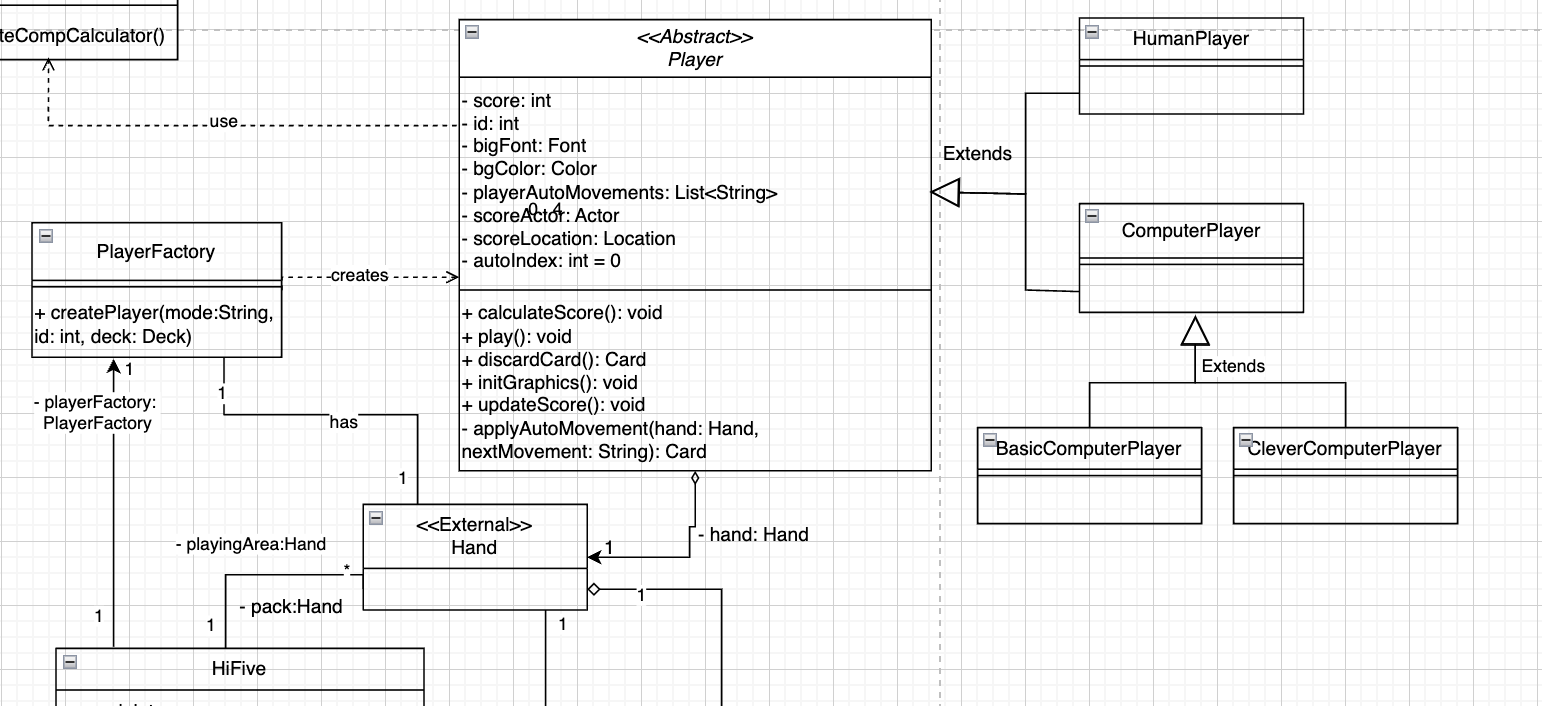
\includegraphics[width=1\linewidth]{player.png}
        \caption{Player Entities implementation}
        \label{fig:enter-label}
    \end{figure}
    % Factory Pattern
    \subsection{Use of Factory Pattern}
    To improve the initialisation process of player entities, we applied the Factory Pattern through the introduction of a '\textbf{PlayerFactory}' class. The Factory Pattern facilitates the creation of different player types such as '\textbf{HumanPlayer}', '\textbf{BasicComputerPlayer}', and '\textbf{CleverComputerPlayer}'. By using a '\textbf{PlayerFactory}', we encapsulate the instantiation logic and keep it separate from the core gameplay code, promoting modularity and reducing code duplication. The '\textbf{PlayerFactory}' class contains a '\textbf{createPlayer()}' method that takes the player's mode, ID, and the deck to instantiate the corresponding player entity. This allows the code to be extendable with new player types while ensuring a uniform way of creating them.
    
    % Pure fabrication
    \subsection{Pure Fabrication and Information Expert Principles}
    The '\textbf{PlayerFactory}' class is a good example of a pure fabrication, meaning that it doesn't represent a concept from the problem domain but is rather a utility class introduced to achieve better modularity. The factory method is also in line with the Information Expert principle of GRASP, where the responsibility for creating player entities is assigned to a dedicated class. This makes the HiFive class simpler and focuses on game control logic instead of also handling player creation.
    
    % Inheritance
    \subsection{Inheritance on Player Classes}
    We refactored the player-related functionality into an abstract class, 'Player', which provides a shared set of properties and methods applicable to all players. The Player class serves as a base, and different player behaviors are implemented through inheritance in derived classes such as '\textbf{HumanPlayer}' and '\textbf{ComputerPlayer}'. The '\textbf{ComputerPlayer}' class is further extended to provide specialized player types like '\textbf{BasicComputerPlayer}' and '\textbf{CleverComputerPlayer}'.

    This use of inheritance not only reduces code duplication but also enables polymorphism, where each player type can implement its play() method in a way that best fits its strategy. This results in better code organization, where player-specific behaviors are encapsulated within their respective classes.

    \subsection{Separation of Player Logic and Gameplay}
    In the refactored version, the responsibility for actions related to player decisions and behavior (such as scoring, discarding cards, and taking turns) is now fully encapsulated within the '\textbf{Player}' classes. Previously, all such logic was cramped within a monolithic '\textbf{HiFive}' class, leading to high coupling and poor readability. By breaking these responsibilities into separate classes, each class now has a single responsibility, aligning with the Single Responsibility Principle. This refactoring also ensures that adding or modifying player behavior is much simpler, as changes are limited to a single class without unintended side effects elsewhere in the code.

    \newpage

    \section{Scoring Algorithms Handling}
    \begin{figure}[htbp]
        \centering
        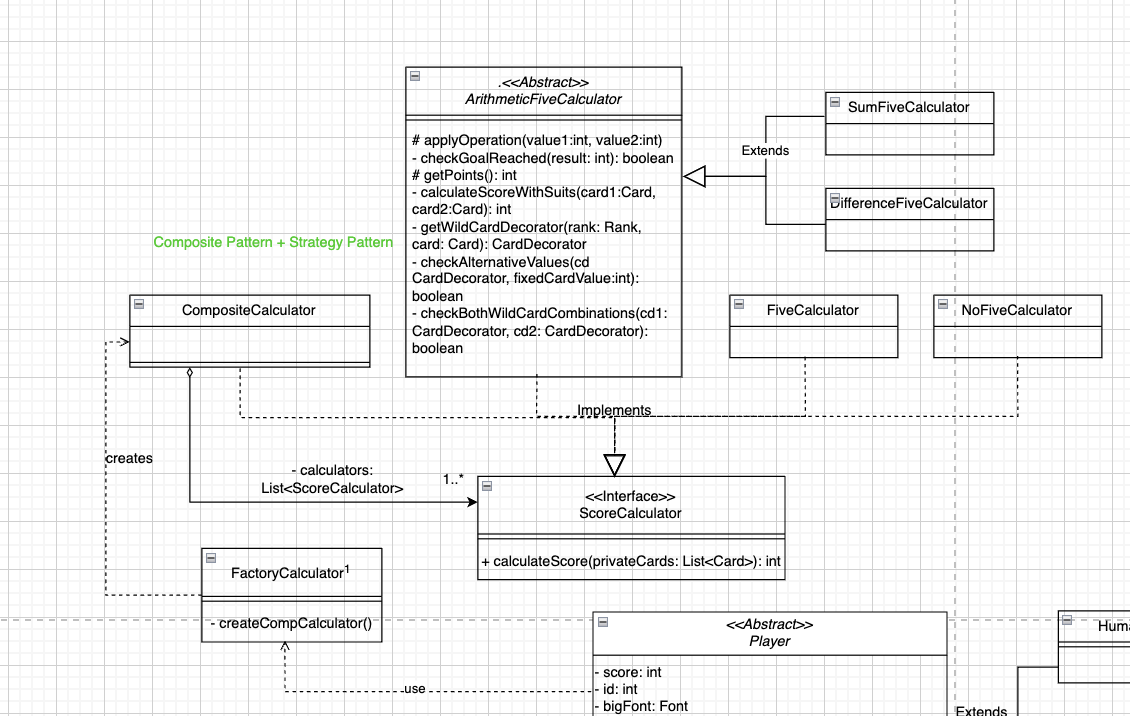
\includegraphics[width=1\linewidth]{Scoring.png}
        \caption{Scoring Algorithm Entities}
        \label{fig:enter-label}
    \end{figure}
    
    % Strategy Pattern
    \subsection{Use of Strategy Pattern}
    
    To handle different scoring rules, we applied the Strategy Pattern to encapsulate four different scoring algorithms: \textbf{FiveCalculator}, \textbf{SumFiveCalculator}, \textbf{DifferenceFiveCalculator}, and \textbf{NoFiveCalculator}. Each of these classes implements the \textbf{ScoreCalculator} interface, which defines a common method for calculating scores. The Strategy Pattern allows us to easily switch between different scoring rules based on the current game situation, making the system more flexible and adaptable. This approach also makes it easy to add new scoring rules in the future, as new strategies can simply be added by implementing the \textbf{ScoreCalculator} interface.
    
    % Composite Pattern
    \subsection{Use of Composite Pattern}
    In order to determine the highest possible score for each player in a round, we need to apply all four scoring algorithms and select the maximum score. For this purpose, we used the Composite Pattern to create a \textbf{CompositeCalculator} class that contains a list of \textbf{ScoreCalculator} objects, including all individual scoring calculators. The \textbf{CompositeCalculator} is responsible for delegating the score calculation to each individual calculator and determining the highest score.
    
    The Composite Pattern helps us to manage multiple score calculators as a single entity, which makes it easier to add or remove scoring algorithms in the future. Moreover, it decouples the scoring logic from the \textbf{Player} classes, resulting in a more modular and reusable design. By delegating the scoring calculation to the \textbf{CompositeCalculator}, the \textbf{Player} class is simplified, as it only needs to interact with the composite to get the final score, rather than managing multiple scoring mechanisms directly.
    
    \subsection{Integration with ArithmeticFiveCalculator}
    We introduced an abstract class, \textbf{ArithmeticFiveCalculator}, that provides common functionality for scoring calculations involving arithmetic operations, such as sums and differences of card values. The \textbf{SumFiveCalculator} and \textbf{DifferenceFiveCalculator} extend \textbf{ArithmeticFiveCalculator}, inheriting the shared methods for calculating and verifying card values, while providing specific implementations for their respective scoring rules. This use of inheritance promotes code reuse and helps to avoid duplication of common logic across different score calculators.

    \subsection{Singleton on FactoryCalculator}
    In order to ensure consistency between calculators and the calculator factory, and reduce memory usage, we applied the Singleton Pattern to the \textbf{FactoryCalculator} class, which is responsible for creating calculators. By implementing the Singleton Pattern, we ensure that there is only one instance of the \textbf{FactoryCalculator} throughout the application, which guarantees that all calculators are created consistently and avoids unnecessary memory consumption.

    \newpage

    \section{Wild Card Functionalities Implementation}    

    \begin{figure}[htbp]
        \centering
        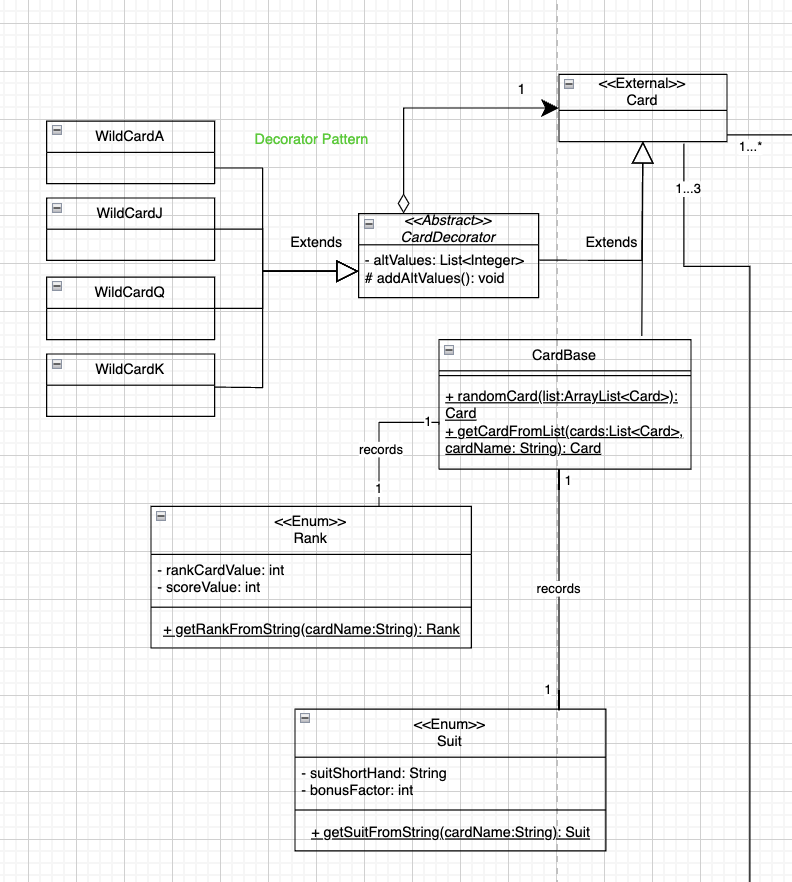
\includegraphics[width=0.8\linewidth]{Cards.png}
        \caption{Design Model Diagram for Wild Cards Part}
        \label{fig:enter-label}
    \end{figure}

    \subsection{Use of Decorator Pattern}
    To implement the Wild Card functionalities in the HiFive game, we used the Decorator Pattern. The Decorator Pattern allows us to add new behaviors to existing card objects without modifying their original code, adhering to the \textit{open-closed principle} of software design. By applying this pattern, we were able to enhance regular card instances with new characteristics that represent wild cards, thereby adding alternative values to the cards.

    The \textbf{CardDecorator} class serves as the abstract decorator, extending the base Card class. It introduces a new property, \textbf{altValues}, which stores the list of possible alternative values for a decorated card. This enables the cards to take on multiple values based on game rules, making them more versatile in different scoring situations.\textbf{}

    The specific wild cards, such as \textbf{WildCardA}, \textbf{WildCardJ}, \textbf{WildCardQ}, and \textbf{WildCardK}, extend from \textbf{CardDecorator} and override methods to provide additional value configurations based on game requirements.

    \subsection{Integration with CardBase and Enum Classes}

    The \textbf{CardBase} class contains utility methods to interact with card objects. These methods facilitate the selection of cards during the game, regardless of whether they are decorated as wild cards or not.

    To further standardize card values, the Rank and Suit classes are implemented as Enums. They help define specific properties like rankCardValue and bonusFactor for card suits, which are used for calculating scores. The Decorator Pattern works seamlessly with these enumerations to provide additional values when calculating scores with wild cards.
    
    \newpage

    % Clever Computer Player Implementation
    \chapter{Clever Computer Player Implementation}

    The Clever Computer Player in the HiFive game aims to make intelligent decisions that maximize the overall score in each turn, following a strategic and computationally efficient approach.

    \section{Approach Overview}
    
    \subsection{Limited Scope of Probability Consideration}
    
    The HiFive game only lasts for four rounds, and each player initially receives two cards, leading to a relatively small number of cards being played in total. Specifically, there are 51 cards available in a deck after removing the jokers, and at most, 16 cards are discarded over the course of four rounds (four players discarding one card each per round).

    Given the limited rounds and high variability in cards dealt, we chose not to consider the cards played by all players when determining the best strategy. The cards in each player's hand are dealt randomly, and attempting to track and predict the remaining cards would significantly increase the game's complexity without adding much value to the player's decision-making. Thus, the Clever Computer Player uses the cards available in its hand to make decisions, without considering broader probability calculations.

    \subsection{Greedy Algorithm for Card Selection}
    
    We adopted a \textbf{greedy algorithm} to maximize the score in the current round based on the cards held by the player. Specifically, the Clever Computer Player uses the following strategy:

    \begin{enumerate}
        \item From the three cards in its hand, the player selects the best two cards that produce the highest score when combined. The third card is discarded.
        \item The approach aims to ensure that in each round, the Clever Computer Player retains the combination of cards most likely to yield the highest score, given the rules of the HiFive game.
    \end{enumerate}
    
    This greedy strategy allows the player to make optimal local decisions without trying to plan across multiple rounds, which aligns well with the limited scope and random nature of card distribution in the game.

    \section{Implementation Details}

    \begin{figure}[htbp]
        \centering
        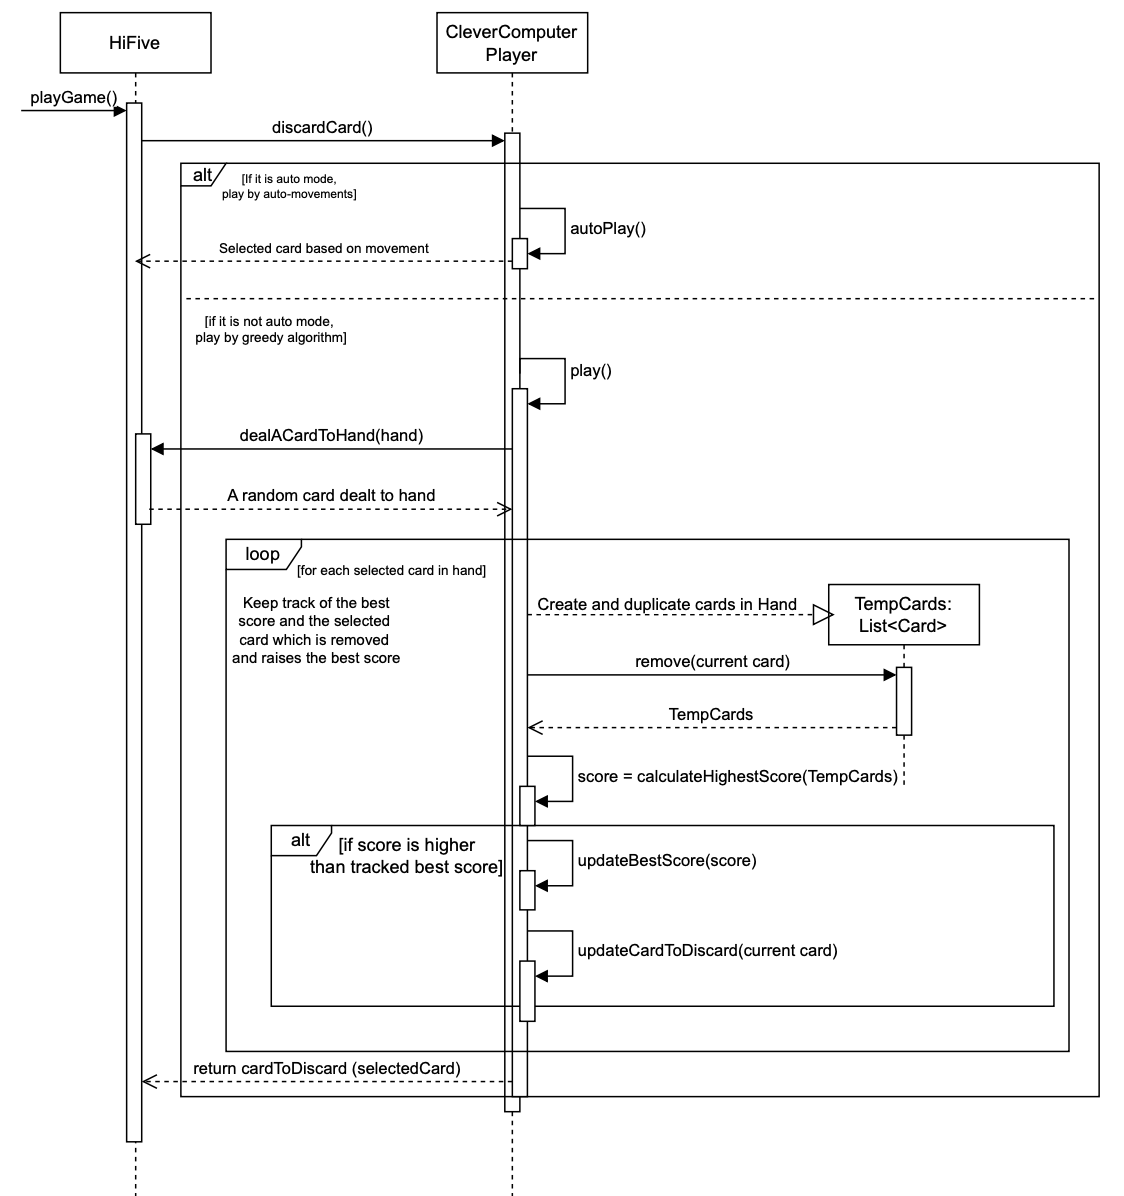
\includegraphics[width=1\linewidth]{Clever.png}
        \caption{Design Sequence Model for Clever Computer Players}
        \label{fig:enter-label}
    \end{figure}
    
    The Clever Computer Player is implemented as a subclass of the \textbf{ComputerPlayer} class, inheriting the basic properties and behavior while extending its logic with a custom \textbf{play()} method that defines the player's decision-making process.

    \subsection{Simulating Card Discard and Score Calculation}
    \begin{enumerate}
        \item The \textbf{play()} method begins by dealing a card from the deck and adding it to the player's hand.
        \item For each card in the hand, the player simulates discarding the card and calculates the potential score that can be achieved using the remaining cards.
        \item The score is calculated using the \textbf{CompositeCalculator}, which applies all four scoring algorithms and determines the maximum score possible with the given combination of cards.
    \end{enumerate}

    \section{Benefits of the Approach}
    \subsection{Maximization of Current Score}
    By using the greedy algorithm, the Clever Computer Player ensures that it always discards the card that is least beneficial for the current round, thereby maximizing the potential score. This approach is well-suited to the short, four-round structure of the game, where each decision has a significant impact on the final outcome.
    \subsection{Simplicity and Efficiency}
    The algorithm focuses on making decisions based solely on the current hand, without considering the broader game state. This reduces computational complexity, allowing the player to make decisions quickly and efficiently. Given the random nature of card dealing, this approach strikes a balance between strategic decision-making and computational feasibility.
    
    \newpage

    % Conclusion
    \chapter{Conclusion}
    The refactoring and extension of the HiFive game code have significantly enhanced the maintainability, flexibility, and overall design quality of the game. By breaking down the original monolithic class into smaller, specialized classes and applying appropriate design patterns, the code is now more modular, adheres to object-oriented principles, and is easier to extend. The introduction of the Clever Computer Player showcases the effectiveness of applying strategic algorithms to maximize game performance in a simplified yet efficient manner. Overall, the improvements have transformed the HiFive game from a poorly structured implementation to a well-designed, flexible, and more engaging system. Based on the robust design choices made during this refactoring process, future enhancements can be more easily integrated.
    
    
\end{document}